\documentclass[12pt]{standalone}
\usepackage{tikz}
%\usetikzlibrary{calc, arrows.meta, decorations.pathreplacing}

\begin{document}

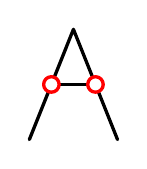
\begin{tikzpicture}[line width=1.2pt, line cap=round, line join=round, scale=1.4]
		% A
		\draw[shorten <= 3.2pt, shorten >= 3.2pt] (0.2,0.5) -- (0.4,1) -- (0.6,0.5);
		\draw[shorten <= 3.2pt, shorten >= 3.2pt] (0.2,0.5) -- (0.6,0.5);
		\draw[shorten <= 3.2pt] (0.2, 0.5) -- (0, 0);
		\draw[shorten <= 3.2pt] (0.6, 0.5) -- (0.8, 0);
		\draw[red] (0.2,0.5) circle(2pt);
		\draw[red] (0.6,0.5) circle(2pt);
	\end{tikzpicture}
\end{document}
